\section{Neutron slowing down}

We want to understand the energy spectrum of neutrons slowing down. We will start by assuming there is only hydrogen around, then we will add in other materials, and finally include heterogeneity in the system. By the end, we should have a pretty good estimate of the neutron spectrum in an LWR geometry.

First, let's define some of the familiar variables in nuclear engineering. 
\begin{itemize}
    \item The scalar flux, $\phi(\mathbf{r},E)$ (where $\mathbf{r}$ is the position and $E$ is the energy), the total track length of neutrons per unit volume or the neutron density times speed $\phi = n\times v$. It has units of neutrons cm$^{-2}$eV$^{-1}$s$^{-1}$.
    \item Macroscopic cross sections, $\Sigma_x(\mathbf{r},E)$, for some reaction type $x$. These are the probability per unit path length that a neutron will undergo some reaction. They have units of cm$^{-1}$. The common reaction types are fission (f), scattering (s), capture (c), absorption (a = f + c), and total (t = a + s). The total cross section is sometimes denoted as simply $\Sigma$.
    \item Microscopic cross sections, $\sigma_x(E)$. These are the target size that a given nucleus presents to a neutron for a given reaction type, with units of cm$^2$. Multiplying by the local density of its corresponding nuclide will give that nuclide's macroscopic cross section, $\Sigma_x = \sigma_x \times N$.
\end{itemize}
With these, we can define other quantities. Reaction rates [s$^{-1}$] in a given volume and energy range are defined as:
\begin{equation*}
    R_x = \int_V \mathrm{d}V \int^{E_1}_{E_2}\mathrm{d}E \;\Sigma_x(E)\phi\;\mathrm{.}
\end{equation*}
For the purposes of our present analysis, we will use reaction rate \textbf{densities}, i.e., not integrated over any part of phase space. For example, the collision rate density (or just the collision density) [collisions cm$^{-3}$ s$^{-1}$ eV$^{-1}$] is given as:
\begin{equation*}
    F(\mathbf{r},E) = \Sigma_\mathrm{t}(\mathbf{r},E)\phi(\mathbf{r},E)\;\mathrm{.}
\end{equation*}

With this we can start analysing slowing down from a  simple case and then build up complexity.

\subsection{Case 1: slowing down on hydrogen}
\textbf{Assumptions:}
\begin{itemize}
    \item There is \textbf{no absorption}, $\Sigma_\mathrm{a} = 0$.
    \item \textbf{Infinite medium}, no leakage.
    \item \textbf{Homogeneous medium}, no dependence of variables on $\mathbf{r}$ (or $\mathbf{\Omega}$).
    \item \textbf{Homogeneously distributed source} $S(E)$ [neutrons cm$^{-3}$ s$^{-1}$ eV$^{-1}$].
    \item \textbf{Elastic scattering on hydrogen} only and $P(E_1\rightarrow E_2) = 1/E_1$ ($\alpha = 0$). This also implies no up-scattering.
\end{itemize}
Some of these assumptions aren't too bad. For example, in hydrogen, the ratio of the absorption cross section to the scattering is about 0.014. However, there are usually more materials nearby which do indeed absorb neutrons.

If we plug all of these assumptions into the transport equation (or just compare our reaction rates) we would end up with:
\begin{equation}
    \Sigma_\mathrm{s}(E)\phi(E) = \int^{\infty}_E\mathrm{d}E'\;\Sigma_\mathrm{s}(E'\rightarrow E)\phi(E') + S(E)\;\mathrm{.}
\end{equation}
Our differential scattering cross section can be divided into its cross section component, $\Sigma_\mathrm{s}(E')$ and its scattering distribution component, $P(E'\rightarrow E)$. From kinematics we had that
\begin{equation*}
    P(E'\rightarrow E)\mathrm{d}E = \frac{\mathrm{d}E}{E'(1-\alpha)}\;\mathrm{,}
\end{equation*}
so our slowing down equation becomes:
\begin{equation*}
    \Sigma_\mathrm{s}(E)\phi(E) = \int^{\infty}_E\mathrm{d}E'\;\frac{\Sigma_\mathrm{s}(E')\phi(E')}{E'} + S(E)\;\mathrm{.}
\end{equation*}
We can also think about this distribution as the probability that a neutron born at $E'$ will scatter into some interval $\mathrm{d}E$ between $E'$ and $\alpha E'$, shown in Fig.~\ref{fig:probdE}. Due to the uniform probability distribution, the probability that a neutron will scatter into a given $\mathrm{d}E$ about $E$ within the range $\alpha E'$ to $E'$ can be thought of as the ratio of these two areas:
\begin{equation*}
    P(E'\rightarrow E)\mathrm{d}E = \frac{A}{B} = \frac{\mathrm{d}E}{E' - \alpha E'}\;\mathrm{.}
\end{equation*}

\begin{figure}[h]
  \centering
  \includegraphics[scale=0.7]{./Figures/P2/probdE.png} 
  \caption{Probability that a neutron scatters into a given energy interval.} 
  \label{fig:probdE}
\end{figure}

Next, we will assert that our neutron source is \textbf{monoenergetic}, i.e., $S(E) = S_0 \delta(E-E_0)$, where $\delta(...)$ is the Dirac delta distribution and $E_0$ is the source energy. We will also introduce the \textbf{collision rate density} $F(E) = \Sigma_\mathrm{s}(E)\phi(E)$ to make things more compact. Thus the slowing down equation becomes:
\begin{equation}\label{eq:slowdown_0}
    F(E) = \int^{E_0}_E\mathrm{d}E'\;\frac{F(E')}{E'} + S_0\delta(E-E_0)\;\mathrm{,}
\end{equation}
where the upper bound of neutron energy is now $E_0$, because neutrons cannot reach higher energies than the source.

The following is hand-wavy, but it's the only way I know how to solve this without resorting to integral equation theory -- what we will do is essentially rewrite Eq.~\eqref{eq:slowdown_0} to remove neutrons that haven't collided and get rid of the delta source. Let's consider the balance of neutrons that make it into some energy interval $\mathrm{d}E$ about energy $E$. These can have come from two sources:
\begin{itemize}
    \item \textbf{Source neutrons that have undergone one collision}. These neutrons are born at energy $E_0$ at a rate of $S_0$ and then scatter once. Since $P(E_0\rightarrow E)\mathrm{d}E = \mathrm{d}E/E_0$, we have this source as:
    \begin{equation*}
        \text{Contribution from first-collided neutrons} = \frac{S_0\;\mathrm{d}E}{E_0}
    \end{equation*}
    \item  \textbf{Source neutrons that have undergone more than one collision}. The source of neutrons is $F(E')\mathrm{d}E'$ for $E' > E$. The number of these neutrons undergoing collisions in an interval $\mathrm{d}E'$ about $E'$ and slowing down to $E$ is:
    \begin{equation*}
        \text{Contribution from previously collided neutrons}= \frac{F(E')\mathrm{d}E'\,\mathrm{d}E}{E'}\;\mathrm{.}
    \end{equation*}
    This squared differential expression represents neutrons in the differential width $\mathrm{d}E'$ about $E'$ scattering into the differential width $\mathrm{d}E$ about $E$.
\end{itemize}
 Hence, our balance in the interval $\mathrm{d}E$ about $E$ becomes:
\begin{equation*}
    F(E)\mathrm{d}E = \frac{S_0\;\mathrm{d}E}{E_0} + \int^{E_0}_E\frac{F(E')\mathrm{d}E'\,\mathrm{d}E}{E'}\;\mathrm{,}
\end{equation*}
or
\begin{equation}\label{eq:slowdown_trick}
    F(E) = \frac{S_0}{E_0} + \int^{E_0}_E\frac{F(E')\mathrm{d}E'}{E'}\;\mathrm{.}
\end{equation}
Differentiating both sides gives:
\begin{equation*}
    \frac{\mathrm{d}F(E)}{\mathrm{d}E} = -\frac{F(E)}{E}\;\mathrm{,}
\end{equation*}
which has the solution:
\begin{equation*}
    F(E) = \frac{C}{E}\;\mathrm{,}
\end{equation*}
for some constant $C$. Inserting this solution into the governing equation at $E=E_0$ gives:
\begin{equation*}
    \frac{C}{E_0} = \frac{S_0}{E_0} + \underbrace{\int_{E_0}^{E_0}\frac{F(E')}{E'}\,dE'}_{=0} = \frac{S_0}{E_0}\;\mathrm{,}
\end{equation*}
so $C = S_0$ and hence:
\begin{equation*}
    F(E) = \frac{S_0}{E}\;\mathrm{,}
\end{equation*}
\begin{equation}\label{eq:Fermi}
    \phi(E) = \frac{S_0}{\Sigma_\mathrm{s}(E)E}\;\mathrm{.}
\end{equation}
We can also write this in terms of lethargy. Noting that $u=\ln(E_0/E)$, $\mathrm{d}u = -\mathrm{d}E/E$, and that $|F(u)\mathrm{d}u| = |F(E)\mathrm{d}E|$ we would get:
\begin{equation*}
    F(u) = F(E) \left|\frac{\mathrm{d}E}{\mathrm{d}u}\right| = E F(E)\;\mathrm{,}
\end{equation*}
or
\begin{equation*}
    \phi(u) = \phi(E) E = \frac{S_0}{\Sigma_\mathrm{s}(u)}\;\mathrm{.}
\end{equation*}
This is why when producing an energy-integrated or multi-group flux (either by deterministic methods or Monte Carlo) the spectrum will tend to be approximately flat in the resonance region.

If we were to be more thorough, we would also obtain an additional $S_0\delta(E-E_0)$ term, i.e., the flux spectrum is strongly influenced by the source close to source energies. However, far from the source, Eq.~\eqref{eq:Fermi} holds and is known as the \textbf{Fermi spectrum} or the \textbf{asymptotic spectrum}.

This might appear an unfriendly equation still due to the dependence upon $\Sigma_\mathrm{s}(E)$. However, in hydrogen, the scattering cross section is a relatively weak function of energy across a large energy range of interest. This is because the cross section is dominated by `potential scattering', i.e., elastic scattering where the cross section corresponds to an effective nuclear radius of the nucleus in question -- which should be constant. The cross section of hydrogen is shown in Fig.~\ref{fig:XS_H}, where the potential scattering's dominance can be seen in the wide range over which the cross section is roughly constant. 

\begin{figure}[h!]
  \centering
  \includegraphics[scale=0.38]{./Figures/P2/hydrogen_XS.jpeg} 
  \caption{The hydrogen microscopic cross section.} 
  \label{fig:XS_H}
\end{figure}

\begin{figure}[h!]
  \centering
  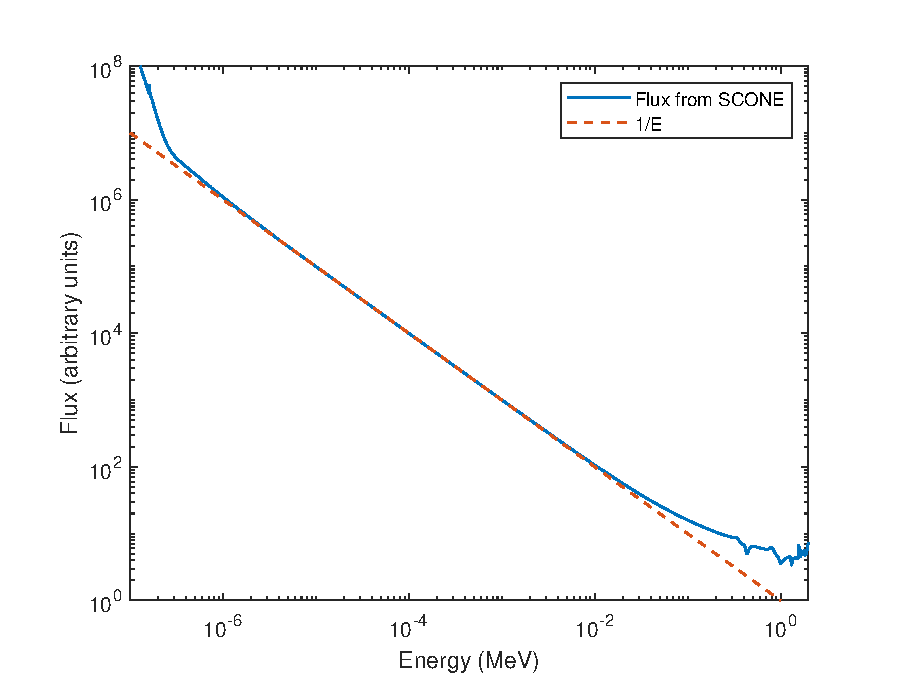
\includegraphics[scale=0.70]{./Figures/P2/fermi.eps} 
  \caption{The spectrum produced by a Monte Carlo code compared to the asymptotic spectrum.} 
  \label{fig:fermi}
\end{figure}

Assuming this constant cross section, this implies the spectrum should look like $\phi(E)\propto 1/E$. This is a remarkably good approximation in reactors far (in energy) from neutron sources. By way of proof, I present in Fig.~\ref{fig:fermi} a spectrum produced by a Monte Carlo code, SCONE, with a source of neutrons at 2 MeV, slowing down in water, as well as the $1/E$ line. For a quite large energy range there appears to be considerable agreement!


But, naturally, the better we approximate the spectrum, the more accurate our final cross sections will be and there are many effects yet to be considered. Cynics might also suggest that you can hide an elephant inside a log-log plot!

Before proceeding, it's useful to investigate the \textbf{neutron slowing down density}, $q(E)$. This is the rate at which neutrons slow down below energy $E$. Formally, this can be calculated as:
\begin{equation*}
    q(E) = \int^{E_0}_E\left[\int^E_0\mathrm{d}E''\;\Sigma_\mathrm{s}(E'\rightarrow E'')\phi(E')\right]\mathrm{d}E'\;\mathrm{.}
\end{equation*}
Less formally, we can calculate this as the total number of neutrons from the source which slow down below $E$ plus the neutrons between $E$ and $E_0$ which then collide to end up below $E$. This can be aided by looking at the probability distribution of collided neutrons, shown in Fig.~\ref{fig:prob_collide}. For a given neutron at some energy $E'>E$, the probability of slowing down below $E$ must be:
\begin{equation*}
    P(\text{of slowing down below }E) = \frac{\text{reachable energies }<E}{\text{energies }\leq E'}\;\mathrm{.}
\end{equation*}
Because, on scattering in hydrogen, the reachable energies from any starting energy are a uniform distribution below that energy, this probability is simply the geometric ratio of areas:
\begin{equation*}
    P(\text{of slowing down below }E) = \frac{\text{reachable energies }<E}{\text{energies }\leq E'} = \frac{E - 0}{E' - 0} = \frac{E}{E'}\;\mathrm{.}
\end{equation*}
Hence, for neutrons freshly born from the source, the slowing down density contribution is:
\begin{equation*}
    S_0 \times P = S_0 \times \frac{E}{E_0}\;\mathrm{,}
\end{equation*}
while for previously scattered neutrons it is:
\begin{equation*}
    \int^{E_0}_E\mathrm{d}E' F(E')\times \frac{E}{E'}\;\mathrm{,}
\end{equation*}
giving:
\begin{equation*}
    q(E) = \frac{S_0 E}{E_0} + E \int^{E_0}_E\mathrm{d}E' \frac{F(E')}{E'}\;\mathrm{.}
\end{equation*}
Using Eq.~\eqref{eq:slowdown_trick}, this turns into:
\begin{equation*}
    q(E) = E F(E)\;\mathrm{,}
\end{equation*}
and using the definition of $F(E)=S_0/E$ we finally get:
\begin{equation*}
    q(E) = S_0\;\mathrm{.}
\end{equation*}
What this tells us is that at any energy $E$ \textbf{there is no accumulation or loss of neutrons}: all neutrons that are born continually slow down. Obviously this is not entirely physical: in reality things like absorption and up-scattering will start to bite!

\begin{figure}[h]
  \centering
  \includegraphics[scale=0.70]{./Figures/P2/slowdownE.png} 
  \caption{Illustration of the probability of slowing down below energy $E$.} 
  \label{fig:prob_collide}
\end{figure}


\subsection{Case 2: slowing down on moderator with $A > 1$}

If we take the most straightforward next step, things immediately become a bit more complicated. If $A>1$, $\alpha \neq 0$, so a neutron cannot lose all of its energy in a single collision. If we have our neutron source with strength $S_0$ producing neutrons at energy $E_0$, then the lowest energy a neutron can reach after one collision is $\alpha E_0$. After two collisions, the minimum energy is $\alpha^2 E_0$, and so on for $n$ collisions where the energy would be $\alpha^n E_0$. We are going to define and work with the collision density for neutrons which have undergone $n$ collisions, $F_n(E)$. Our logic will be helped by the diagram in Fig.~\ref{fig:slowdown_interval}.

\begin{figure}[h]
  \centering
  \includegraphics[scale=0.60]{./Figures/P2/slowdownA.png} 
  \caption{Illustration of the intervals into which a neutron can slow down into given a number of scattering events.} 
  \label{fig:slowdown_interval}
\end{figure}

We will do this by once again splitting the collision density into its components and we can recover the collision density as $F(E) = \sum^\infty_{n=1}F_n(E)$.
\begin{itemize}
    \item \textbf{Neutrons having undergone 1 collision.} These neutrons will be born with energy $E_0$ and will scatter according to the usual scattering law, but with a different lower energy bound. Hence we would get (multiplying $S_0\delta(E-E_0)$ by $P(E_0\rightarrow E)$ and integrating):
    \begin{equation*}
        F_1(E) =  \left\{\begin{array}{ll}
      \frac{S_0 }{E_0(1-\alpha)}\;\mathrm{;}\;\; \alpha E_0\ < E < E_0\\
      0\;\mathrm{;}\;\; E < \alpha E_0
      \end{array} 
      \right.\;\mathrm{.}
    \end{equation*}
    This function is obviously discontinuous about $\alpha E_0$ and $E_0$.
    \item \textbf{Neutrons having undergone 2 collisions.} These are the neutrons which result from the collision of neutrons produced by $F_1(E)$. They have two possibilities in their lives: scatter and remain in the energy range $\alpha E_0 < E < E_0$ or scatter into the next energy range down, $\alpha^2 E_0 < E < \alpha E_0$. 
    \textbf{Neutrons that remain in the same energy range} can scatter anywhere from $E_0$ down to the energy of interest $E$($>\alpha E_0$):
    \begin{equation*}
        F_2(E) = \int^{E_0}_E\frac{F_1(E')\mathrm{d}E'}{E'(1-\alpha)} = \frac{S_0}{E_0(1-\alpha)^2}\int^{E_0}_E\frac{\mathrm{d}E'}{E'} = \frac{S_0}{E_0(1-\alpha)^2}\ln\left(\frac{E_0}{E}\right)\;\mathrm{;}\;\;\alpha E_0 < E < E_0\;\mathrm{.}
    \end{equation*}
    \textbf{Neutrons that scatter into the lower range} $\alpha^2 E_0 < E < \alpha E_0$ must have a maximum energy of $E' = E/\alpha$. However, from $F_1(E)$, they cannot have an energy lower than $\alpha E_0$. Therefore, we obtain an integral like:
    \begin{equation*}
        F_2(E) = \int^{E/\alpha}_{\alpha E_0}\frac{F_1(E')\mathrm{d}E'}{E'(1-\alpha)} = \frac{S_0}{E_0(1-\alpha)^2}\int^{E/\alpha}_{\alpha E_0}\frac{\mathrm{d}E'}{E'} = \frac{S_0}{E_0(1-\alpha)^2}\ln\left(\frac{E}{\alpha^2 E_0}\right)\;\mathrm{;}\;\;\alpha^2 E_0 < E < \alpha E_0\;\mathrm{.}
    \end{equation*}

    Below $\alpha^2 E_0$, no neutrons can go after only two scatters. So $F_2(E) = 0$ for $E < \alpha^2 E_0$. Therefore, $F_2(E)$ is:
    \begin{equation*}
        F_2(E) = \left\{\begin{array}{lll}
        \frac{S_0}{E_0(1-\alpha)^2}\ln\left(\frac{E_0}{E}\right)\;\mathrm{;}\;\;\alpha E_0 < E < E_0 \\
        \frac{S_0}{E_0(1-\alpha)^2}\ln\left(\frac{E}{\alpha^2 E_0}\right)\;\mathrm{;}\;\;\alpha^2 E_0 < E < \alpha E_0\\
        0\;\mathrm{;}\;\; E < \alpha^2 E_0
        \end{array} 
      \right.\;\mathrm{.}
    \end{equation*}
    While the function is now continuous at all points, it now has a discontinuous derivative at $E = \alpha E_0$. 
    \item As you can imagine, the general expressions for collision densities become even more complicated for $n > 2$ collisions...
\end{itemize}

\begin{figure}[h]
  \centering
  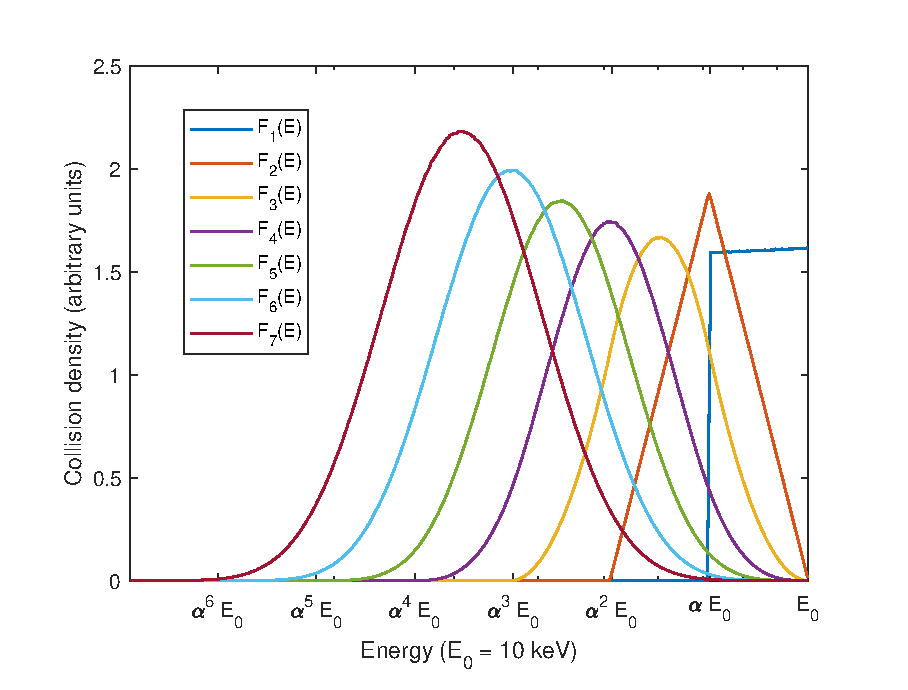
\includegraphics[scale=0.70]{./Figures/P2/placzek_carbon.eps} 
  \caption{The first few collision densities produced from a 10 keV fixed neutron source in graphite (the tilt in $F_1$ is due to some scattering anisotropy).} 
  \label{fig:placzek}
\end{figure}

Fortunately, not only does $F_n(E)$ become more smooth as $n\rightarrow \infty$, but, far from the source, $F(E)$ once again obtains a $1/E$ shape! Solving a fixed source graphite problem in SCONE, the first few of these collision densities (or Placzek distributions) are shown in Fig.~\ref{fig:placzek}. The usual approximation is to say for $E < \alpha^3 E_0$ we can solve the following equation by asserting that the source has little influence:
\begin{equation*}
    F(E) \approx \int^{E/\alpha}_{E}\frac{F(E')\mathrm{d}E'}{E'(1-\alpha)}\;\mathrm{.}
\end{equation*}
It is easy to show that $F(E) = C/E$ is a solution by plugging it in -- it is much harder to show that it is the only solution! Finding the constant, $C$, takes a little bit of work. One way to do this is to use our previous knowledge that, in a non-absorbing problem, $q(E) = S_0$; we then need to find what $q(E)$ is for $\alpha \neq 0$. We do this in a similar manner as before by phrasing the problem in terms of slowing down from one energy and reaching another:
\begin{equation*}
    P\left(\text{slow down below }E\right) = \frac{E - \alpha E'}{E' - \alpha E'} = \frac{A}{B}\;\mathrm{.}
\end{equation*}
This is illustrated in Fig.~\ref{fig:prob_collide_alpha}.

\begin{figure}[h]
  \centering
  \includegraphics[scale=0.70]{./Figures/P2/probCollideAlpha.png} 
  \caption{Illustration of the probability of slowing down below energy $E$ given limits on maximum energy loss.} 
  \label{fig:prob_collide_alpha}
\end{figure}

From before, our definition of $q(E)$ is:
\begin{equation*}
    q(E) = \int^{E/\alpha}_E \mathrm{d} E' F(E')P(\text{slow down below }E) = \int^{E/\alpha}_E \mathrm{d}E' \frac{C}{E'} \frac{E - \alpha E'}{E' - \alpha E'} = C\left(1 + \frac{\alpha}{1-\alpha}\ln\alpha\right) = C\xi = S_0\;\mathrm{.}
\end{equation*}
Here we remember $\xi$ as the average lethargy gain per collision. Hence:
\begin{equation*}
    F(E) = \frac{S_0}{\xi E}\;\mathrm{;}\; \phi(E) = \frac{S_0}{\xi \Sigma_\mathrm{s} E}\;\mathrm{.}
\end{equation*}
Hence, once again, the Fermi spectrum holds.

\subsection{Case 3: Non-monenergetic source}

Sources in nuclear reactors are not monoenergetic and this will affect the validity of the equations we obtain, but thankfully not too much. 

Recall that the equations we have from before,
\begin{equation*}
    \phi(E) = \frac{S_0}{\Sigma_\mathrm{s}E} \;\text{for }A = 1\; \mathrm{,}
\end{equation*}
and
\begin{equation*}
    \phi(E) = \frac{S_0}{\xi\Sigma_\mathrm{s}E} \;\text{for }A > 1\;\mathrm{,}
\end{equation*}
are the solutions for the slowing down source $S_0\delta(E-E_0)$ -- otherwise known as Green's functions. This means that the generalisation is simply to integrate over whatever source distribution we have, $S(E)$, giving:
\begin{equation*}
    \phi(E) = \frac{1}{\Sigma_\mathrm{s}E} \int^\infty_{E_\mathrm{cut}}\mathrm{d}E'\;S(E')\;\text{for }A = 1\; \mathrm{,}
\end{equation*}
and
\begin{equation*}
    \phi(E) = \frac{1}{\xi\Sigma_\mathrm{s}E} \int^\infty_{E_\mathrm{cut}}\mathrm{d}E'\;S(E')\;\text{for }A > 1\;\mathrm{.}
\end{equation*}
Usually we do not integrate between $0$ and $\infty$, but rather from some lower bound, $E_\mathrm{cut}$. This is often taken to be about 50 keV. Below this value only about 1\% of fission neutrons are produced and we would expect the asymptotic spectrum to be reached due to the weak source.

\subsection{Case 4: Slowing down in a mixture of nuclides}

Let's denote a given nuclide with index $i$ such that we can define:
\begin{equation*}
    F^{(i)}(E)\text{: collision density on nuclide }i
\end{equation*}
\begin{equation*}
    \Sigma^{(i)}_\mathrm{s}(E)\text{: scattering cross section of nuclide }i
\end{equation*}
This lets us write:
\begin{equation*}
    F^{(i)}(E) = \Sigma^{(i)}_\mathrm{s}\phi(E) \times \frac{\Sigma_\mathrm{s}(E)}{\Sigma_\mathrm{s}(E)} = \frac{\Sigma^{(i)}_\mathrm{s}(E)}{\Sigma_\mathrm{s}(E)} \times F(E)\;\mathrm{.}
\end{equation*}
We also have that the equation for $F(E)$ is simply:
\begin{equation*}
    F(E) = \sum_i \int^{E/\alpha_i}_E\frac{\mathrm{d}E' F^{(i)}(E')}{E'(1-\alpha_i)}\;\mathrm{.}
\end{equation*}
We will look for solutions of the form $F^{(i)}(E) = C_i/E$ -- this should satisfy the previous equation, but it does not tell us the value of $C_i$. Lacking absorption, we still have that $q(E) = S$ where $S = S_0$ for a point energy source or $S=\int\mathrm{d}E S(E)$ for a spectrum. The expression for $q(E)$ is:
\begin{equation*}
\begin{split}
    q(E) = \sum_i \int^{E/\alpha_i}_{E}F^{(i)}(E) \times \frac{E-\alpha_i E'}{E' - \alpha_i E'}\mathrm{d}E' = \sum_i \int^{E/\alpha_i}_{E}\frac{C_i}{E} \times \frac{E-\alpha_i E'}{E' - \alpha_i E'}\mathrm{d}E'\\
    = \sum_i C_i \left(1 + \frac{\alpha_i}{1-\alpha_i}\ln\alpha_i\right) = \sum_i C_i \xi_i = S\;\mathrm{.}
    \end{split}
\end{equation*}
We also have another expression for $C_i$, which we can insert, namely $C_i = F^{(i)}E$:
\begin{equation*}
    S = \sum_i C_i\xi_i = E\sum_i F^{(i)}\xi_i = E F(E) \sum_i \frac{\Sigma^{(i)}_\mathrm{s}(E)}{\Sigma_\mathrm{s}(E)}\xi_i\;\mathrm{.}
\end{equation*}
If we define
\begin{equation*}
    \bar{\xi}(E)= \frac{\sum_i \xi_i \Sigma^{(i)}_\mathrm{s}(E)}{\Sigma_\mathrm{s}(E)}\;\mathrm{,}
\end{equation*}
then:
\begin{equation*}
    S = EF(E)\bar{\xi}(E)\;\mathrm{,}
\end{equation*}
\begin{equation*}
    F(E) = \frac{S}{\bar{\xi}(E) E}\;\text{;  } \phi(E) = \frac{S}{\bar{\xi}(E)\Sigma_\mathrm{s}(E) E}\;\mathrm{.}
\end{equation*}

\subsection{Case 5: Slowing down with absorption}

We'll revert back to a point energy source, $S_0\delta(E-E_0)$, where $E_0$ is above the resonance region such that there is no absorption on first collision. Suppose we have a mix of purely scattering hydrogen and heavy absorber with $A\rightarrow \infty$ (so we can drop $\alpha$ from our scattering energy distributions). 

The balance of neutrons becomes:
\begin{equation*}
    F(E)\mathrm{d}E = \text{neutrons arriving in }\mathrm{d}E\text{ after 1 collision} + \text{neutrons arriving into }\mathrm{d}E\text{ after }>1\text{ collision}\;\mathrm{.}
\end{equation*}
From before, the first term is going to be simply:
\begin{equation*}
    \text{Neutrons arriving into }\mathrm{d}E\text{ after 1 collision} = S_0 \frac{\mathrm{d}E}{E_0}\;\mathrm{,}
\end{equation*}
while the second term will be produced from $F(E')\mathrm{d}E'$ which then \textbf{survive the collision} and \textbf{get scattered to }$E$. The probability of surviving a collision is given by:
\begin{equation*}
    \frac{\Sigma_\mathrm{s}(E)}{\Sigma_\mathrm{t}(E)} = \frac{\Sigma_\mathrm{s}(E)}{\Sigma_\mathrm{s}(E) + \Sigma_\mathrm{a}(E)}\;\mathrm{,}
\end{equation*}
while getting redistributed to $E$ is the usual $\mathrm{d}E/E'$. Hence:
\begin{equation*}
    \text{Neutrons arriving into }\mathrm{d}E\text{ after }>1\text{ collision}= \int^{E_0}_E F(E')\frac{\Sigma_\mathrm{s}(E')}{\Sigma_\mathrm{s}(E') + \Sigma_\mathrm{a}(E')}\frac{\mathrm{d}E'}{E'}\mathrm{d}E\;\mathrm{.}
\end{equation*}
Hence, the equation for the collision density is:
\begin{equation}\label{eq:F_abs}
    F(E) = \frac{S_0}{E_0} + \int^{E_0}_E F(E')\frac{\Sigma_\mathrm{s}(E')}{\Sigma_\mathrm{s}(E') + \Sigma_\mathrm{a}(E')}\frac{\mathrm{d}E'}{E'}\;\mathrm{.}
\end{equation}
As before, we will differentiate to get:
\begin{equation*}
    \frac{\mathrm{d}F(E)}{\mathrm{d}E} = -\frac{F(E)}{E}\frac{\Sigma_\mathrm{s}(E)}{\Sigma_\mathrm{s}(E) + \Sigma_\mathrm{a}(E)}\;\mathrm{.}
\end{equation*}
Using the balance of probabilities, we can convert the scatter probability into $1 - $ absorption probability:
\begin{equation*}
    \frac{\Sigma_\mathrm{s}(E)}{\Sigma_\mathrm{s}(E) + \Sigma_\mathrm{a}(E)} = 1 - \frac{\Sigma_\mathrm{a}(E)}{\Sigma_\mathrm{s}(E) + \Sigma_\mathrm{a}(E)}\;\mathrm{.}
\end{equation*}
This allows us to rewrite the collision density differential equation to give:
\begin{equation*}
    \frac{\mathrm{d}F(E)}{F(E)} = -\frac{\mathrm{d}E}{E} + \frac{\Sigma_\mathrm{a}(E)}{\Sigma_\mathrm{s}(E) + \Sigma_\mathrm{a}(E)}\frac{\mathrm{d}E}{E}\;\mathrm{,}
\end{equation*}
giving, when integrating from $E$ to $E_0$:
\begin{equation*}
    \ln\left(\frac{F(E_0)}{F(E)}\right) = -\ln\frac{E_0}{E} + \int^{E_0}_E\frac{\Sigma_\mathrm{a}(E')}{\Sigma_\mathrm{s}(E') + \Sigma_\mathrm{a}(E')}\frac{\mathrm{d}E'}{E'}\mathrm{,}
\end{equation*}
and:
\begin{equation*}
    F(E) = \frac{F(E_0)E_0}{E}\exp\left(-\int^{E_0}_E\frac{\Sigma_\mathrm{a}(E')}{\Sigma_\mathrm{s}(E') + \Sigma_\mathrm{a}(E')}\frac{\mathrm{d}E'}{E'}\right)\;\mathrm{.}
\end{equation*}
This means that $q(E)$ is no longer uniform across energy because $q(E) = F(E)E \neq F(E_0)E_0$. This is because of absorption. The expression for $q(E)$ in this case is:
\begin{equation*}
    q(E) = \frac{S_0E}{E_0} + E\int^{E_0}_E \frac{\Sigma_\mathrm{s}(E')}{\Sigma_\mathrm{s}(E') + \Sigma_\mathrm{a}(E')}\frac{F(E')\mathrm{d}E'}{E'}\;\mathrm{.}
\end{equation*}
Note that from this we can equate $F(E_0)E_0 = S_0$ with the integral reducing to 0. Also recall $q(E)$ is the number of neutrons that survived slowing down to energy $E$. Hence we can speak of a probability of not being absorbed:
\begin{equation}\label{eq:res_escape_prob}
    p(E) = \frac{q(E)}{S} = \exp\left(-\int^{E_0}_E\frac{\Sigma_\mathrm{a}(E')}{\Sigma_\mathrm{s}(E') + \Sigma_\mathrm{a}(E')}\frac{\mathrm{d}E'}{E'}\right)\;\mathrm{.}
\end{equation}
This is the \textbf{resonance escape probability}. To say anything more useful, we need to understand something about how $\Sigma_\mathrm{a}(E)$ and $\Sigma_\mathrm{s}(E)$ look, in particular with respect to resonant behaviour.

